\chapter{Discussion}

\section{Hardware Performance}
Controls development and hardware operation for this drive was severely
hampered by a poor choice in inter-module connectors and lack of test-points.
As such, full vector-control was never realized.  Several important results
however were able to be measured.

\subsection{Current Sensors}
The open-field hall effect current sensors on this prototype performed
admirably both in providing nicely filtered signals and having interference
from neighboring phases attenuated below what the system could measure.

The current sense amplitude response is shown in Fig.
\ref{figCurrentResponse}.
This shows a roll off in amplitude above 1kHz.
In a typical system this would be a problem due to phase lag, however this
roll off is due to field shaping as the higher-frequency components of the
magnetic field from the phase bar are concentrated near the edges of the phase
conductor \cite{Schneider10}.
This gives the advantage that we can have switching frequency current
components attenuated while still having nearly lag-free response.

\begin{figure}[htbp]
	\centering
	\label{figCurrentResponse}
	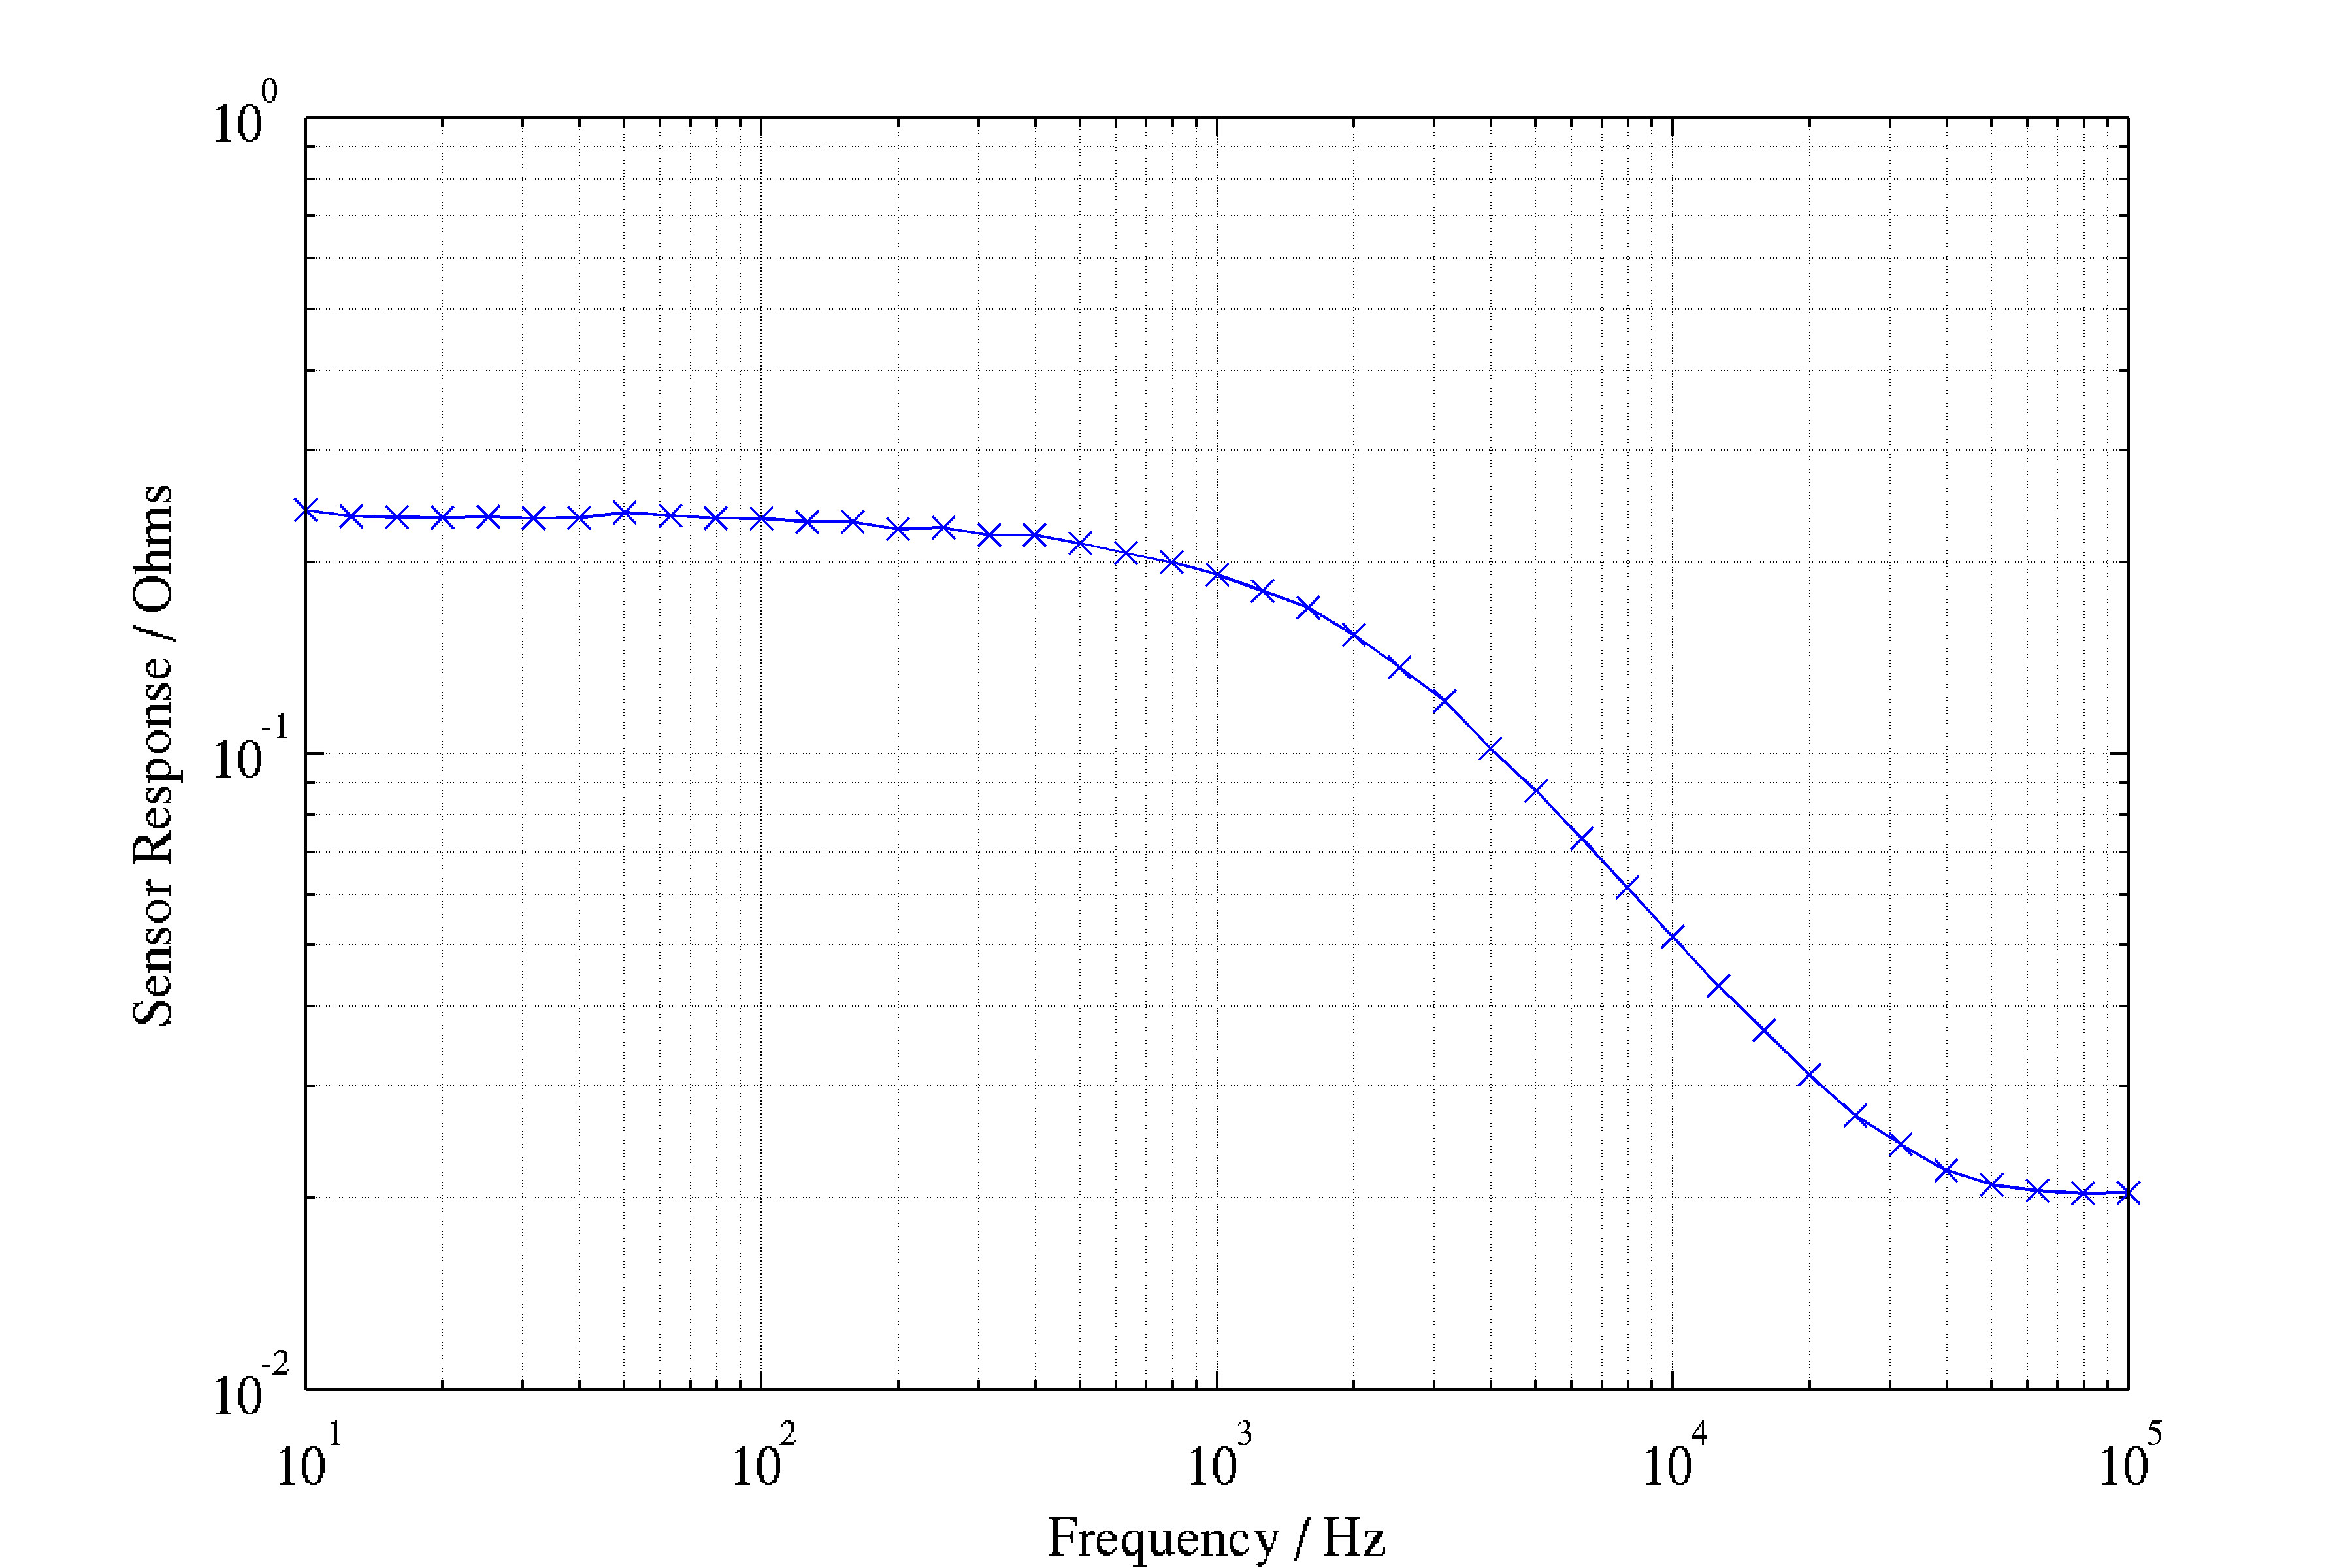
\includegraphics[width=\textwidth]{CurrentSense}
	\caption{Current sensor gain response.  Vertical units are ADC input voltage
	over phase current.  The ADC operates on a 1.65V full scale.}
\end{figure}

\subsection{Motor Operation}
Due to cost, the motor used in this prototype has a 3x overlength rotor.  This
causes a significant increase in PM flux and brings the characteristic current
to nearly 3pu.
This machine decision was made after the converter was partially built and as
such, the converter cannot survive fault transients at significant speed or
full voltage.

The motor was thus operated at reduced voltage and brought up to just below
its design corner speed of 2400rpm.  Using V/Hz operation, the drive was able
to run the machine smoothly operating with independent control of all six
phases.  The waveforms for one phase are shown in Fig. \ref{figWaveform}.

\begin{figure}[htbp]
	\centering
	\label{figWaveform}
	\includegraphics[width=\textwidth]{\detokenize{IMMD_VHz_200}}
	\caption{Waveforms for 2400rpm, V/Hz operation.}
\end{figure}

\section{Scaling}
A study was made of scaling the drive up to the full 55kW design required by
the USDrive specification.

In that case, the only significant change would be a tripling of the capacitor
size and a replacement of the power module component with a higher current
device.
Semikron and Infineon both supply 600V 300A modules in a similar footprint to
the TO-247 based design used in this prototype thus no further increase in
volume is needed for the power switches.
Our waterblock design also has significant cooling capacity overhead.

The capacitor resize would essentially double the size of the inverter as the
current inverter volume is dominated by the waterblock and capacitor.
Table \ref{tabSizing} shows an overview of the volumetric and mass density of
the prototype converter and upsized versions in both pancake arrangement where
the drive covers the end of the machine rotor and annular where the drive
footprint remains the same but the axial length is doubled.
